% !TeX spellcheck = id_ID
\documentclass[a4paper,12pt]{article}
\usepackage[bahasa]{babel}
\usepackage{graphicx}
\usepackage{multirow}
\usepackage{enumitem}
\usepackage{listings}
\usepackage{wrapfig}
\usepackage[T1]{fontenc}
\usepackage{inconsolata}
\usepackage{lipsum}
\usepackage{adjustbox}


\usepackage{color}
\usepackage[table]{xcolor}
\definecolor{pblue}{rgb}{0.13,0.13,1}
\definecolor{pgreen}{rgb}{0,0.5,0}
\definecolor{pred}{rgb}{0.9,0,0}
\definecolor{pgrey}{rgb}{0.46,0.45,0.48}
\lstset{language=Java,
	showspaces=false,
	showtabs=false,
	breaklines=true,
	showstringspaces=false,
	breakatwhitespace=true,
	commentstyle=\color{pgreen},
	keywordstyle=\color{pblue},
	stringstyle=\color{pred},
	rulecolor=\color{black},
	basicstyle=\ttfamily,
	moredelim=[il][\textcolor{pgrey}]{$$},
	moredelim=[is][\textcolor{pgrey}]{\%\%}{\%\%}
}

\graphicspath{ {./img/} }
\begin{document}
\title{ {\Large Laporan Praktikum}\\ Algoritma dan Pemrograman \\{\Large Pertemuan 10}}

\author{Aldzikri Dwijayanto Prathama 
	\\195410189
	\\Teknik Informatika}
\makeatletter
\begin{titlepage}
	\begin{center}
		{\huge \bfseries \@title }\\[14ex]
		
\includegraphics[scale=.8]{logo}\\[4ex]
		{\large \@author}\\[19ex]
		{\large \bfseries {SEKOLAH TINGGI MANAJEMEN INFORMATIKA DAN KOMPUTER
				AKAKOM YOGYAKARTA}}
	\end{center}


%{\large \@date} 
\end{titlepage}
\makeatother
%\maketitle
\newpage
\tableofcontents
\newpage

\section{Tujuan}
Mahasiswa dapat mengimplementasikan konsep perulangan do-while untuk menyelesaikan kasus

\section{Dasar Teori}
\paragraph{}
Perintah  pengulangan  ini  digunakan  untuk  mengulangi  suatu  baris  perintah 
tertentu  dengan  jumlah  pengulangan  yang  sudah  diketahui  sebelumnya,  selain  itu 
perintah pengulangan ini dilengkapi dengan pencacah (counter). Perintah for mempunyai 
tiga  buah  argumen.  Argumen yang  pertama merupakan  deklarasi  dan  pemberian  nilai 
awal variabel, yaitu variabel yang digunakan sebagai pencacah (counter), argumen yang 
kedua (di tengah) pada perintah for ini merupakan suatu kondisi (ekspresi logika) yang 
diuji,  apabila  menghasilkan  nilai  true  maka  perulangan  akan  dilakukan  (dilanjutkan) 
sedangkan jika false maka pengulangan akan dihentikan. Argumen yang ketiga, yaitu yang 
paling  kanan  merupakan  perintah  yang  akan  dieksekusi  setiap  kali  perintah  dalam 
perulangan  dijalankan.  Pada  umumnya  argument  ketiga  ini  berupa  perintah  untuk 
menaikkan  (increment)  atau  menurunkan  (decrement)  nilai  variable  pencacah  yang 
diinisialisasi  pada  argument  pertama.  Nilai  variabel  penghitung  akan  secara  otomatis
bertambah atau berkurang tiap kali sebuah pengulangan20 dilaksanakan tergantung perintah yang ditulis pada argumen ini. \\
Sintaks penulisan perintah for sebagai berikut :
\begin{lstlisting}[frame=single]
for(nilai_awal; ekspresi_logika; penambahan/penurunan)

{
	Pernyataan;
}
\end{lstlisting}
Argumen pertama bisa berupa variable, biasanya bertipe int dan langsung diberi nilai awal, apabila nama variabel sudah dideklarasikan pada baris sebelumnya maka variabel tersebut dapat langsung digunakan dalam perintah for ini dan akan tetap dikenal meskipun keluar dari kalang (loop) yaitu blok perulangan, namun jika dideklarasikan di dalam perintah for, maka identifier variabel tersebut hanya dikenal di dalam kalang dan tidak akan dikenal diluar kalang (setelah perintah for selesai). Argumen yang kedua merupakan ekspresi logika, biasanya berupa pembandingan nilai (memakai operator hubungan/ pembanding) dari variabel yang dideklarasikan pada argument pertama, sedangkan argument yang terakhir berupa perintah increment atau decrement dari variabel yang dideklarasikan pada argument pertama memakai operator unary ++ atau --
Perulangan dalam pemrograman dibagi menjadi dua jenis:
\begin{enumerate}
	\item \textbf{Counted loop}: Perulangan yang jumlah pengulangannya terhitung atau tentu.
	
	\item \textbf{Uncounted loop}: Perulangan yang jumlah pengulangannya tidak terhitung atau tidak tentu.
	
\end{enumerate}	

\begin{center}
	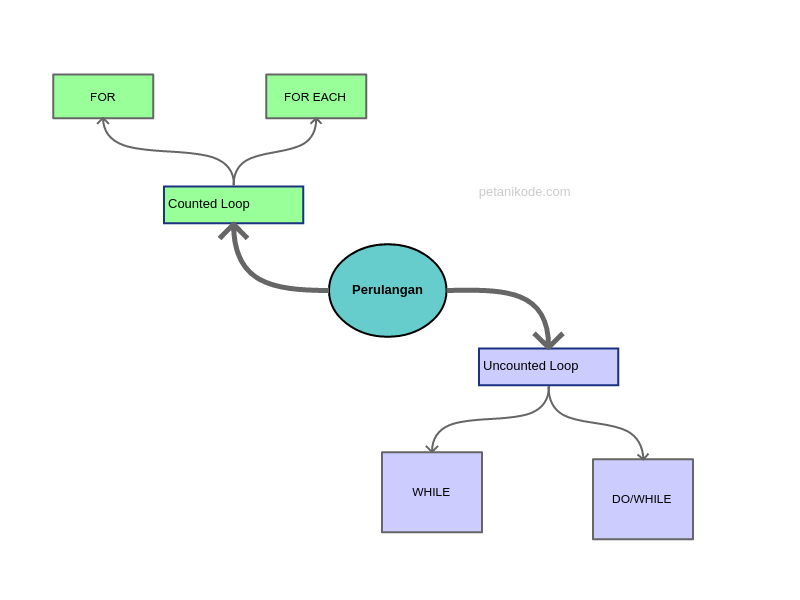
\includegraphics[scale=.45]{mindmap}
\end{center}
Counted loop terdiri dari perulangan For dan For each. Sedangkan Uncounted loop terdiri dari perulangan While dan Do/While

\newpage

\section{Praktik}
\subsection{Praktik 1}
\begin{enumerate}[label=\alph*.]
	\item 
	\begin{minipage}[t]{\linewidth}
		\raggedright
		\adjustbox{valign=t}{
			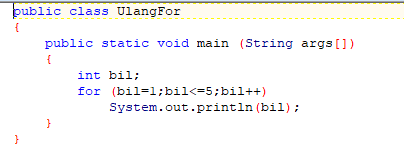
\includegraphics[width=.8\linewidth]{Capture1}%
		}
	\end{minipage}
	Pada program java di atas dituliskan program dengan perulangan for yang memiliki bagian-bagian:
	\begin{itemize}
		\item     variabel bil tugasnya untuk menyimpan hitungan pengulangan.
		\item bil <= 5 artinya selama nilai hitungannya lebih kecil atau sama dengan 5, maka pengulangan akan terus dilakukan. Dengan kata lain, perualangan ini akan mengulang sebanyak 5 kali.
		\item bil++ fungsinya untuk menambah satu (+1) nilai hitungan peda setiap pengulangan.
	
	\end{itemize}
	Blok kode For dimulai dengan tanda ‘{’ dan diakhiri dengan ‘}’.\\
	Jadi program tersebut akan menghitung 1 - 5 dan menge-print nilai variabel bil, sehingga program akan menampilkan angka 1 - 5 di layar, dari atas ke bawah.\\
	Jadi outputnya setelah program dicompile dan dijalankan akan menjadi seperti di bawah
	\begin{center}
		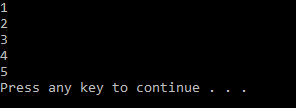
\includegraphics[scale=1]{Capture2}
	\end{center}
	
	\item 
	\begin{minipage}[t]{\linewidth}
		\raggedright
		\adjustbox{valign=t}{
			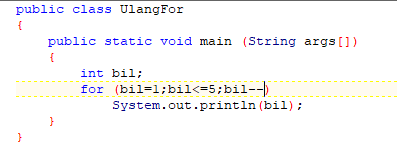
\includegraphics[width=.8\linewidth]{Capture3}%
		}
	\end{minipage}
	Lalu jika bil++ dirubah menjadi bil-- program akan terus berjalan, karena setiap perulangan terjadi kondisinya selalu true, sehingga pengulangan akan terus dijalankan dan menjadi perulangan tak terbatas
	Outputnya setelah program dicompile dan dijalankan seperti berikut.\\
	\begin{center}
		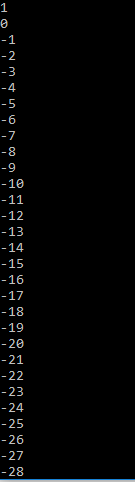
\includegraphics[scale=1]{Capture4}
	\end{center}
\end{enumerate}

\subsection{Praktik 2}
\begin{enumerate}[label=\alph*.]
	\item 
	\begin{minipage}[t]{\linewidth}
		\raggedright
		\adjustbox{valign=t}{
			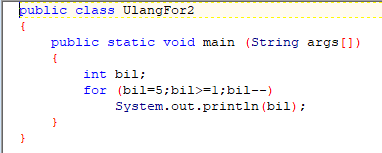
\includegraphics[width=.8\linewidth]{Capture5}%
		}
	\end{minipage}
	Pada program java di atas dituliskan program dengan perulangan for yang memiliki bagian-bagian:
	\begin{itemize}
		\item     variabel bil tugasnya untuk menyimpan hitungan pengulangan dan diberi nilai 5.
		\item bil >= 1 artinya selama nilai hitungannya lebih besar atau sama dengan 1, maka pengulangan akan terus dilakukan. Dengan kata lain, perualangan ini akan mengulang sebanyak 5 kali.
		\item bil-- fungsinya untuk mengurangi satu (-1) nilai hitungan pada setiap pengulangan.
	\end{itemize}
	Jadi program tersebut akan menghitung 5 - 1 dan menge-print nilai variabel bil, sehingga program akan menampilkan angka 5 - 1 di layar, dari atas ke bawah.\\
	Jadi outputnya setelah program dicompile dan dijalankan akan menjadi seperti di bawah
	\begin{center}
		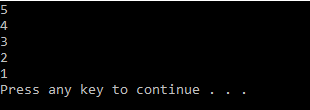
\includegraphics[scale=1]{Capture6}
	\end{center}
	\newpage
	\item 
	\begin{minipage}[t]{\linewidth}
		\raggedright
		\adjustbox{valign=t}{
			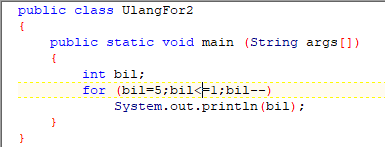
\includegraphics[width=.8\linewidth]{Capture7}%
		}
	\end{minipage}
	Pada program selanjutnya bil>=1 dirubah menjadi bil<=1, hasilnya program akan langsung eluar tanpa melakukan perulangan, karena kondisi yang dinyatakan sudah false.\\
	Outputnya sebagai berikut.
	\begin{center}
		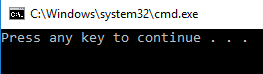
\includegraphics[scale=1]{Capture8}
	\end{center}

	\item 
	\begin{minipage}[t]{\linewidth}
		\raggedright
		\adjustbox{valign=t}{
			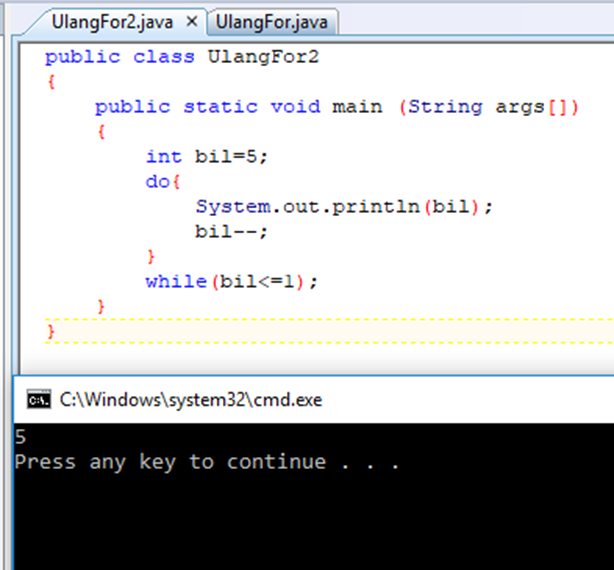
\includegraphics[width=.8\linewidth]{image10}%
		}
	\end{minipage}
	Jika praktik 2b dirubah perulangannya menjadi perulangan do-while maka int bil diberi nilai sendiri, lalu outputnya akan menjadi 5. hal ini karena perulangan do-while akan melakukan pernyataan yang diberikan terlebih dahulu, baru memeriksa kondisi.
	
\end{enumerate}

\subsection{Praktik 3}
\begin{center}
	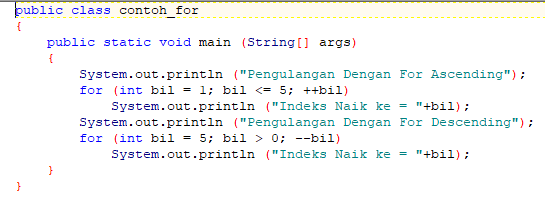
\includegraphics[scale=1]{Capture11}
\end{center}
Program di atas memiliki perulangan for, yang pertama memiliki bagian: 
\begin{itemize}
	\item variabel bil tugasnya untuk menyimpan hitungan pengulangan.
	\item bil <= 5 artinya selama nilai hitungannya lebih kecil atau sama dengan 5, maka pengulangan akan terus dilakukan. Dengan kata lain, perualangan ini akan mengulang sebanyak 5 kali.
	\item bil++ fungsinya untuk menambah satu (+1) nilai hitungan peda setiap pengulangan.
	\item Pernyataan yang akan mngeprint nilai dari variabel bil 
\end{itemize}
jadi perulangan yang pertama akan mengeprint bilangan dari 1 sampai 5.\\
Sedangkan perulangan kedua memiliki bagian seperti berikut:
\begin{itemize}
	\item     variabel bil tugasnya untuk menyimpan hitungan pengulangan dan diberi nilai 5.
	\item bil > 0 artinya selama nilai hitungannya lebih besar atau sama dengan 0, maka pengulangan akan terus dilakukan. Dengan kata lain, perualangan ini akan mengulang sebanyak 5 kali.
	\item bil-- fungsinya untuk mengurangi satu (-1) nilai hitungan pada setiap pengulangan.
\end{itemize}
Jadi fungsi perulangan kedua adalah menampilkan bilangan dari 5 sampai 1.\\
Output dalam konsol adalh seperti berikut:
\begin{center}
	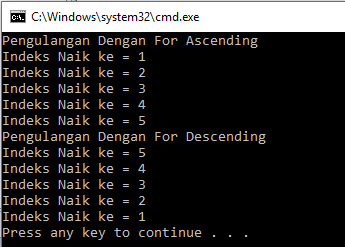
\includegraphics[scale=1]{Capture12}
\end{center} 

\section{Latihan}
\begin{enumerate}
	\item 
	\begin{minipage}[t]{\linewidth}
		\raggedright
		\adjustbox{valign=t}{
			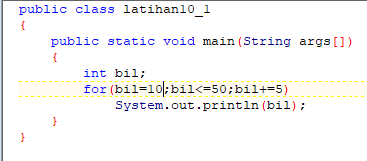
\includegraphics[width=.8\linewidth]{Capture13}%
		}
	\end{minipage}
	Program java tersebut jika dijalankan akan menampilkan bilangan kelipatan 5 dari 10 sampai 50. Jadi perulangannya seperti berikut:
	\begin{itemize}
		\item variabel bil diberi nilai awal 10.
		\item bil <= 50 artinya selama nilai hitungannya lebih kecil atau sama dengan 50, maka pengulangan akan terus dilakukan. Dengan kata lain, perualangan ini akan mengulang sampai variabel bil bernilai 50.
		\item bil+=5 fungsinya untuk menambah lime (+5) nilai hitungan pada setiap pengulangan.
		\item Pernyataan yang akan mngeprint nilai dari variabel bil 
	\end{itemize}
	Jadi outputnya seperti berikut
	\begin{center}
		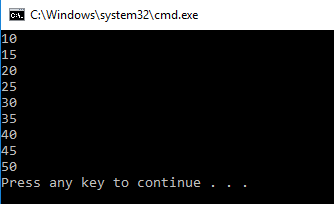
\includegraphics[scale=1]{Capture14}
	\end{center}
	
	\item 
	\begin{minipage}[t]{\linewidth}
		\raggedright
		\adjustbox{valign=t}{
			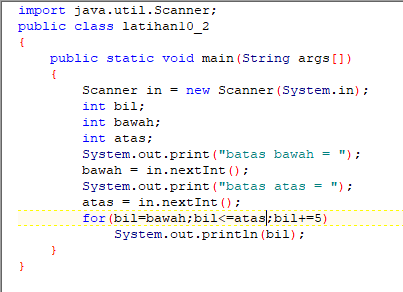
\includegraphics[width=.8\linewidth]{Capture15}%
		}
	\end{minipage}
	Pada program di atas, variabel bawah dan atas variabelnya ditentukan oleh user, lalu variabel bil memiliki nilai sama dengan nilai variabel bawah. Perulangan ini akan terus dilakukan selama variabel bil lebih kecil atau sama dengan nilai di variabel atas. Sehingga program di atas akan menampilkan bilangan kelipatan 5, yang nilai awal dan akhirnya ditentukan oleh user.\\
	Output di konsol adalah seperti berikut.
	\begin{center}
		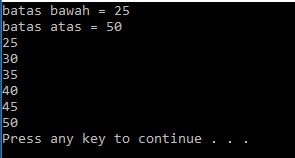
\includegraphics[scale=1]{Capture16}
	\end{center} 
\end{enumerate}

\section{Tugas}
\begin{enumerate}
	\item 
	\begin{minipage}[t]{\linewidth}
		\raggedright
		\adjustbox{valign=t}{
			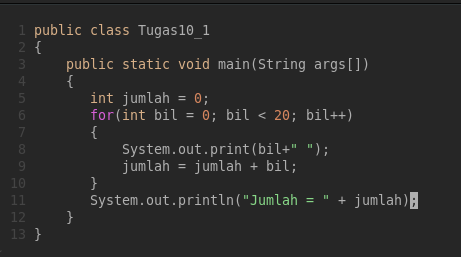
\includegraphics[width=.8\linewidth]{tugas1}%
		}
	\end{minipage}
	Program java tersebut jika dijalankan akan menampilkan bilangan dari 0 sampai 19. Program tersebut memiliki variabel jumlah untuk menampung hasil penjumlahan dari angka yang ditampilkan, dan memiliki perulangan for yang seperti berikut:
	\begin{itemize}
		\item variabel bil diberi nilai awal 0.
		\item bil < 20 artinya selama nilai hitungannya lebih kecil dari 20, maka pengulangan akan terus dilakukan. 
		\item bil++ fungsinya untuk menambah satu (+1) nilai hitungan pada setiap pengulangan.
		\item Pernyataan yang akan mngeprint nilai dari variabel bil 
		\item Pernyataan yang akan memasukkan nilai dari variabel bil, dan menambahkan dengan variabel bil perulangan berikutnya.
	\end{itemize}
	Jadi outputnya seperti berikut
	\begin{center}
		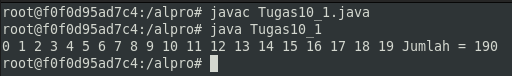
\includegraphics[scale=.7]{tugas1_2}
	\end{center}
	\item 
	\begin{minipage}[t]{\linewidth}
		\raggedright
		\adjustbox{valign=t}{
			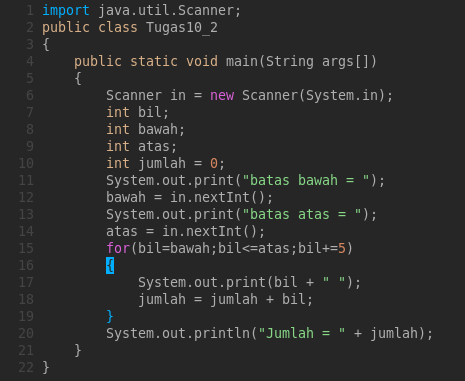
\includegraphics[width=.8\linewidth]{tugas2}%
		}
	\end{minipage}
	Jika program dari latihan 1 dirubah agar bisa menjumlahkan bilangan yang ditampilkan maka ditambahkan variabel jumlah untuk menyimpan hasil penjumlahan, dan ditambahkan pernyataan yang akan memasukkan nilai dari variabel bil ke variabel jumlah, dan menambahkan dengan variabel bil perulangan berikutnya.\\
	Output dalam konsol seperti berikut:
	\begin{center}
		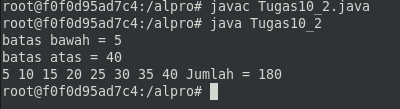
\includegraphics[scale=.8]{tugas2_2}
	\end{center}
\end{enumerate}

\newpage
\section{Kesimpulan}
Setelah praktik ini mahasiswa dapat mengimplementasikan konsep perulangan do-while untuk menyelesaikan kasus


\end{document}